%\documentclass[12pt]{scrreprt}
\documentclass[12pt]{report} 

% language may be romanian or english (default is english)
% type may be bachelor or master (default is bachelor)
\usepackage[language=romanian, type=bachelor]{style}

%\geometry{a4paper,top=2.5cm,left=3cm,right=2.5cm,bottom=2.5cm}
%in style
%controlling the appearance of your headers and footers
\usepackage{fancyhdr}
\usepackage{graphicx}
\usepackage{float}
\usepackage{svg}
\usepackage{combelow}
\usepackage[utf8]{inputenc}
\usepackage[T1]{fontenc}
\usepackage{listings}
\usepackage{courier}
\usepackage{vcell}
\usepackage{caption}
\usepackage{subcaption}
\pagestyle{fancy}
\lhead{}
\chead{}
\renewcommand{\headrulewidth}{0.2pt}
\renewcommand{\footrulewidth}{0.2pt}
\lstset{basicstyle=\ttfamily, breaklines=true}

% Attributes for preventing the overlapping of the text written with monospace font (\texttt)
\tolerance=1
\emergencystretch=\maxdimen
\hyphenpenalty=10000
\hbadness=10000

\begin{document}

\specialization{INFORMATICĂ}	
\title{Distribuția streamurilor audio-video în sesiuni WebRTC}					   
\author{Haja Florin-Gabriel}											
\supervisor{Lect. dr. Sterca Adrian-Ioan}				
				
\maketitle


\newpage
\thispagestyle{empty}
\mbox{}


\newpage
\pagenumbering{roman} 

\cleardoublepage
ABSTRACT
\vspace{0.5cm}	
\hrule
\vspace{0.5cm}	
%\cleardoublepage

%\par Această lucrare este un studiu în profunzime al protocoalelor de comunicare folosite de proiectul WebRTC și al modului în care conținutul audio-video poate fi distribuit în cadrul a mai multor clienți. Odată ce oamenii folosesc Internetul în scop productiv din ce în ce mai mult, este crucială asigurarea faptului că informația este transmisă pe cât de fluent posibil. Deoarece unele conexiuni la Internet au o lățime de bandă limitată, este mai dificilă gestionarea sesiunilor de apel video cu mulți utilizatori.
%\par This thesis is an in-depth study of communication protocols used by
%\par Putem opta ori pentru un server media care să gestioneze livrarea datelor pentru noi, ori pentru a conecta fiecare client cu toți ceilalți, într-o manieră a topologiei mesh (engl. plasă). De exemplu, în cadrul participării la un curs, se poate observa un scenariu de broadcasting, în care profesorul furnizează conținutul, iar studenții doar îl observă, așadar datele sunt transmise într-o singură direcție, iar topologia mesh nu are un beneficiu real. În locul servirii tuturor studenților deodată, putem servi câțiva, aceștia trimițând repetat streamul mai departe, până când toți pot să vizioneze ceea ce predă profesorul. Se poate observa o topologie arborescentă. Nu mai este nevoie de un server media, însemnând costuri de mentenanță mai mici, cu un compromis din partea clienților al lățimii de bandă folosite.

\par This thesis is an in-depth study of the communication protocols used by the WebRTC project and the way the audio-video content can be distributed across multiple clients. As people are using the Internet productively more and more, it is crucial to ensure the information is transmitted as fluidly as possible. Since some Internet connection may be limited in bandwidth, it is more difficult to handle video call sessions with many users. 
\par We can opt for using a media server that handles the data delivery for us, or to connect each client with the other, in a mesh topology fashion. When attending a class, for example, we are noticing a broadcasting scenario, as the teacher is providing the content and the students are only looking at it, thus the data can be streamed in one direction, and the mesh topology having no real purpose. Instead of serving all the students at once, we can serve a few, which will forward the stream to others, repeatedly streaming until everyone is able to watch what is the teacher showing. We notice a tree topology. A media server is no longer required, meaning cheaper maintenance costs, but sacrificing the low bandwidth each client is using.


\tableofcontents
\listoffigures


\newpage
\pagenumbering{arabic}

%\addcontentsline{toc}{chapter}{Introducere}
%\addcontentsline{toc}{chapter}{Introduction}

\chapter{Introducere}
\label{intro}
\chapter{Istoria conferințelor video}
\label{sec:ch2}

\section{Era analogică}
\label{sec:ch2sec1}

\indent \par Primele concepte ale transmiterii de imagini datează încă din secolul XIX, contemporane cu brevetarea telefonului de către Alexander Graham Bell în data de 14 februarie 1876 și prezentarea acestuia la Expoziția Centenară de la Philadelphia în același an. Un articol publicat în 30 martie 1877 de către The New York Sun menționează termenul \textit{electroscop} în acest context, prin care prezintă posibilele aplicații ale unui dispozitiv prin care se pot observa imagini din orice colț al lumii. De asemenea, scriitori precum Abbé Moigno și Louis Figuier, prezintă un concept foarte similar, creând termenul \textit{telectroscop}, atribuindu-i-l eronat lui Graham Bell \cite{Electroscope1878, Telectroscope1877}. 
\begin{figure}[b]
    \centering
    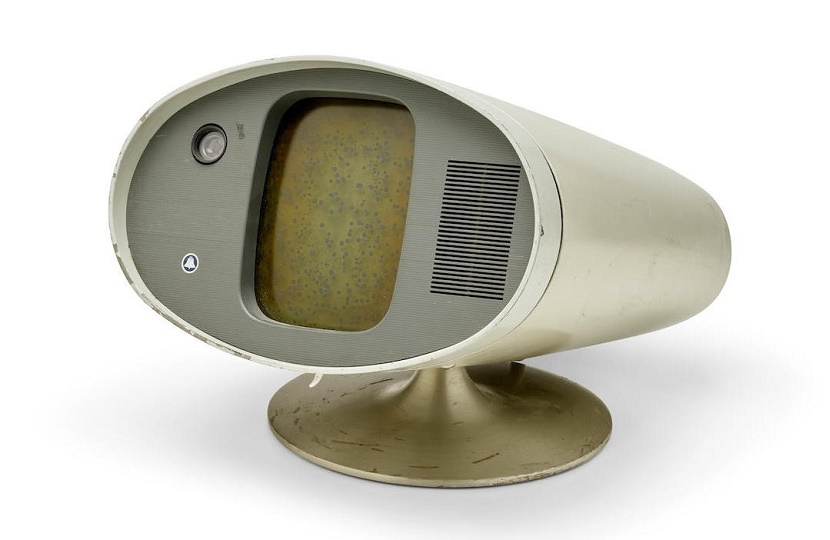
\includegraphics[width=6.99cm]{figures/picturephone.jpg}
    \caption{Primul model de Picturephone, care a fost instalat în cabine în 3 orașe din Statele Unite}
\end{figure}
\indent \par Însă primul prototip funcțional a fost demonstrat public în 7 aprilie 1927 într-o aulă din New York. Herbert Hoover, pe atunci secretarul comerțului al Statelor Unite, a apărut pe ecran din Washington D.C., fiind observat de către oficialii companiei AT\&T \cite{Videophone1927}. Apelul era unidirecțional pentru imagine și bidirecțional pentru sunet, datorită liniilor telefonice deja existente. Mai târziu, la Expoziția Mondială de la New York din 1964, AT\&T a prezentat primul Picturephone, la care publicul putea să efectueze apeluri bidirecționale către o cabină telefonică similară montată la Disneyland, folosind conexiune VHF sau UHF prin cablu \cite{Avoira2020}. Acesta a fost indisponibil pentru uz casnic până în 1970, când aceeași companie a lansat un Picturephone îmbunătațit, disponibil printr-un serviciu lunar. Din cauza costului ridicat de 160 de dolari pe lună (echivalent a 1000 de dolari în 2020), nu a prezentat interes, serviciul fiind desființat în 1973 \cite{Videophone1927}.

\section{Era digitală și tranziția către Internet}
\label{sec:ch2sec2}

\indent \par În anii '80, diverse companii, printre care Mitsubishi, au comercializat diverse videotelefoane care puteau transmite imagini statice prin intermediul rețelei telefonice deja existente, fapt care permitea folosirea modemurilor existente cu rate de transfer între 2,4 și 9,6 kilobiți pe secundă. Evoluția algoritmilor digitali de compresie a imaginilor și a lățimii de bandă, a permis ca AT\&T să mai încerce o dată cu VideoPhone 2500, care, de asemenea, nu a avut succes, costând inițial 1500 de dolari în 1992 \cite{Borth98}.
\indent \par Apariția protocoalelor Internet și a tehnicilor și mai avansate de compresie audio-video a permis ca imaginea și sunetul să fie transmise în pachete mult mai mici, rezultând în costuri mult mai reduse. Simultan cu dezvoltarea rețelei ARPANET (precursoarea Internetului), destinată inițial pentru transfer de date, s-a discutat problema comunicării în timp real prin voce \cite{RFC741}. Așadar, s-a propus în decembrie 1973 implementarea Network Voice Protocol (NVP), care a venit cu următoarele considerente: separarea semnalelor de control de traficul de date, evitarea retransmiterii pachetelor pierdute, adaptabilitate la condițiile variabile ale rețelei, precum și independența gestionării resurselor de către fiecare sistem, dar și de către protocoalele de nivel mai jos\cite{RFC741}.
\indent \par PictureTel a jucat un rol important în evoluția comunicațiilor video. Cei doi fondatori ai săi, Brian L. Hinman și Jeffrey G. Bernstein, absolvenți ai MIT și buni prieteni, au fondat PicTel în 1984 (a fost ulterior redenumită pentru a evita confuzia cu termenul \textit{pixel}) cu sprijin financiar din partea lui Robert Sterling. În 1986, după ce compania a devenit publică, a dezvoltat algoritmul Motion Compensated Transform (MCT), care a permis reducerea unei transmisii audio-video de calitate de la 768 Kb/s la 224. Pe baza acestui algoritm, au lansat codecul C-2000 în luna iulie al aceluiași an, cu ajutorul căruia PictureTel a devenit lider în domeniul său. În 1988, un nou algoritm de compresie video a fost lansat, Hierarchical Vector Quantizing (HVQ), folosit în codecul C-3000, precum și în sistemul V-2100 \cite{Root2000}. Cu ajutorul acestuia, lățimea de bandă folosită a fost redusă la jumătate, comparativ cu algoritmul MCT. În anii '90, a colaborat la crearea standardului H.320 pentru videoconferințe prin rețeaua ISDN, precum și a standardului H.323 pentru comunicare audio-video prin Internet pe baza protocolullui TCP, cel din urmă folosit pentru a crea produsul software LiveLan \cite{Root2000}.
\indent \par O dată cu migrarea videoconferințelor către Internet, au început să apară soluții gratuite, potrivite și consumatorilor de rând, care să nu ceară echipament auxiliar, pe lângă un computer și o cameră web. Una din primele aplicații influente de acest fel este realizată de Tim Dorcey la Universitatea Cornell și se numește CU-SeeMe, apărut prima dată în 1992 pentru sistemele Macintosh \ref{CUSeeMeMac}. Apelurile cu doi participanți pot fi inițiate de către unul din ei conectându-se direct la celălalt, în timp ce apelurile cu mai mulți participanți necesită conectarea fiecăruia la un \textit{reflector} CU-SeeMe \cite{Dorcey95}. \textit{Reflectorul} este un software destinat sistemelor UNIX ce are menirea de a a redistribui fluxurile de pachete, principala sa motivație fiind lipsa abilităților de multicast pe Macintosh de la vremea respectivă \cite{Dorcey95}. Pentru transmisie, imaginea se împarte în pătrate de dimensiune 8x8, acestea fiind selectate pentru trimitere doar în cazul în care gradul de similitudine este suficient de ridicat \cite{Dorcey95}. Acest grad este calculat ca sumă a tuturor diferențelor absolute între fiecare pixel de pe aceeași poziție, la care se aplică o penalizare multiplicativă pentru diferențele între pixelii apropiați \cite{Dorcey95}. Mai târziu, a adoptat standardul H.323, care s-a regăsit și pe alte produse, precum Microsoft NetMeeting (începând cu versiunea 2) \cite{Vidconf, Perey2000}.
\begin{figure}[H]
    \centering
    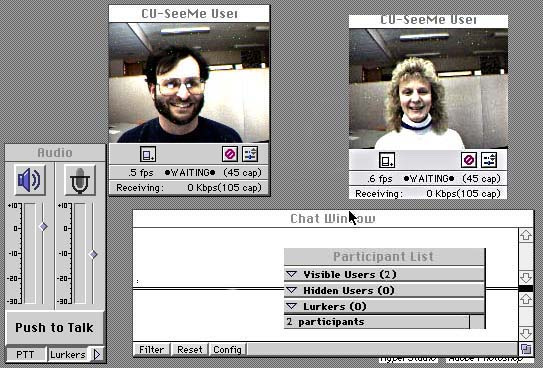
\includegraphics[width=9.1cm]{figures/cu-seeme.jpg}
    \caption{Aplicația CU-SeeMe rulând pe Macintosh}
    \label{CUSeeMeMac}
\end{figure}
\indent \par În 1994, un moment important a fost lansarea primei camere web destinate consumatorilor, Connectix QuickCam \ref{QuickCam} \cite{Wolfe2019}. Putea captura imagini doar în 16 culori la 15 cadre pe secundă și a fost inițial compatibilă doar cu Macintosh \cite{Wolfe2019}. Un an mai târziu, a fost lansată și varianta pentru Windows. Însă calitatea redusă a imaginii nu a fost un impediment pentru persoanele aflate la distanță de a se putea simți aproape una de cealaltă, de a putea interacționa, de a trăi evenimente aflate în diverse colțuri ale lumii \cite{QuickCam94}. Ulterior, au apărut variante îmbunătațite de QuickCam, cu captură de imagini color la rezoluții mai mare, dar și cu conectivitate paralelă și USB.
\begin{figure}[H]
    \centering
    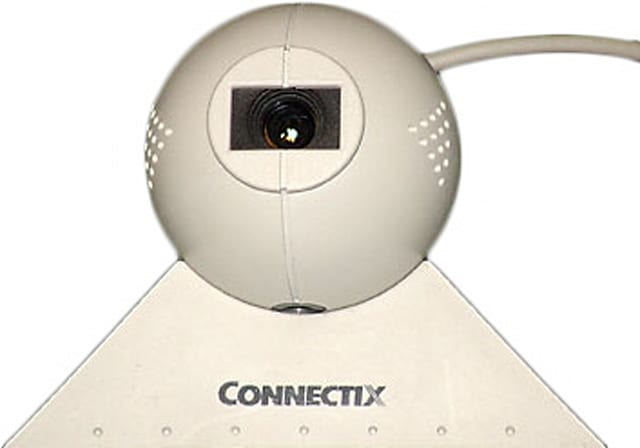
\includegraphics[width=5.7cm]{figures/quickcam.jpg}
    \caption{Connectix QuickCam, prima cameră web comercială}
    \label{QuickCam}
\end{figure}
\indent \par În paralel s-au dezvoltat o multitudine de standarde menite de a reduce și mai mult lățimea de bandă folosită, precum și de a ușura crearea de noi platforme de comunicare. În 1997 a fost creat Session Initiation Protocol (SIP), prin care utilizatori pot fi invitați la participarea într-o sesiune multimedia, sau chiar servere prin care se poate înregistra sesiunea \cite{rfc2543}. Este o combinație dintre Session Invitation Protocol și dintre Simple Conference Invitation Protocol, prin care se încearcă potrivirea lui SIP pe o infrastructură mai flexibilă care include și alte protocoale, precum SDP, HTTP și RTSP \cite{rfc2543}. Poate funcționa atât peste TCP, cât și peste UDP, pentru o performanță îmbunătațită \cite{rfc2543}.
\indent \par Codecurile video au continuat de-a lungul timpului să evolueze. În 2003, Unitatea Internațională a Telecomunicațiilor (ITU - Internation Telecommunication Union) a făcut public standardul H.264, destinat codării audio-video în aplicații precum televiziunea prin cablu și satelit, videoconferințe prin Internet, dar și filme stocate pe medii de stocare optice \cite{H.264}. Folosește tehnici precum partiționarea imaginilor în macroblocuri, precum și codificare predictivă bidirecțională. A fost dezvoltat împreună cu ISO MPEG (Moving Picture Experts Group) \cite{H.264}.
\indent \par Între timp, au apărut platforme de mesagerie instantă precum AOL Instant Messenger (AIM) în 1997, Yahoo! Messenger în 1998, MSN Messenger în 1999 \cite{Wolfe2019}. Toate au suportat apeluri video în 2003, folosind, în principiu, SIP pentru a iniția apelurile și RTP pentru transportul pachetelor. Apple a lansat în 2002 un client pentru AIM numit iChat, folosind implementarea oficială a protocolului furnizată de America Online \cite{Wolfe2019}. iChat a primit suport pentru codecul H.264 în 2004, oferind calitate mai bună decât predecesorul său, H.263 \cite{Royal2007}.
\indent \par Însă mult mai popular pentru apelurile video a devenit Skype, care, când a fost lansat în 2003 de KaZaa, permitea apeluri gratuite în grup de 25 de persoane. Promitea, la momentul respectiv, calitate a vocii superioară față de alternativele Yahoo și MSN, dar și o traversare facilă a NAT-urilor și firewall-urilor \cite{Baset2004}. Singurul rol al serverului central era doar de login, informațiile utilizatorilor fiind păstrate într-o manieră descentralizată, prin intermediul nodurilor și supernodurilor \ref{SkypeNet} \cite{Baset2004}. Un nod ce dispune de suficientă putere de procesare și lățime de bandă fi candidat pentru a fi supernod \cite{Baset2004}. Se presupunea că fiecare nod folosește o variație a protocolului STUN pentru a comunica pe rețeaua suprapusă Skype \cite{Baset2004}. De asemenea, fiecare nod își păstra o listă de supernoduri cu care să facă legătura - această listă este denumită \textit{host cache} și este păstrată în registrul sistemului de operare Windows \cite{Baset2004}. Ulterior, Skype a fost cumpărat de Microsoft în 2011 și a renunțat la topologia cu supernoduri pentru o scalabilitate mai bună, folosind, în schimb, serverele Microsoft, cu toate că au existat suspiciuni privind securitatea serviciului \cite{Whittaker2013}.
\indent \par Apoi, a urmat înglobarea unei colecții de protocoale precum SDP, STUN, TURN și RTP, precum și a unor codecuri precum VP8, G.711 și iLBC într-un proiect numit WebRTC, care vine inclus cu majoritatea browserelor moderne și pe baza căruia s-au construit majoritatea aplicațiilor moderne precum Microsoft Teams, Zoom, Jitsi Meet, OBS.Ninja și inclusiv FaceTime, care s-au dovedit esențiale în mediul profesional și academic pe parcursul epidemiei de coronavirus începută în 2019 și care continuă și în 2021.
\begin{figure}
    \centering
    \scalebox{0.65}{\input{figures/skypenetwork.pdf_tex}}
    \caption{O reprezentare a topologiei de rețea folosită de Skype}
    \label{SkypeNet}
\end{figure}
\chapter{WebRTC}
\label{chap:ch3}

\indent \par Acest capitol are ca scop introducerea în principiile de bază și în componentele proiectului WebRTC, cu menirea de a putea înțelege conceptele următoare. Acoperă API-urile comune, precum și principiile de rețelistică folosite pentru comunicare calitativă, cu latență mică.
\indent \par WebRTC a fost dezvoltat ca standard de către World Wide Web Consortium (W3C) și de către Internet Engineering Task Force (IETF), fiind o colecție open-source de standarde și protocoale. Tehnologiile necesare, precum codecuri și algoritmi de anulare a ecoului, au fost dezvoltate de către o companie suedeză numită Global IP Solutions (GIPS), care a fost mai târziu cumpărată de Google în mai 2010 \cite{WebNSM2017}. Google a făcut publică implementarea acest proiect în mai 2011 și a propus către IETF standardizarea acestuia. Similar, alți lideri ai industriei precum Mozilla, Ericsson, Microsoft și Apple au furnizat implementări pentru WebRTC, în 2013 fiind realizată interoperabilitatea între browserele Chrome și Firefox \cite{Nyman2013}. Standardul a fost finalizat în ianuarie 2021 și este cunoscut ca RFC 8825.

\section{Arhitectura}
\label{sec:ch3sec1}

% TODO modifică partea asta
\subsection{Stabilirea conexiunilor}
\label{sec:ch3sec1subsec1}
\indent \par La începuturile videoconferințelor pe Internet, protocolul dominant pentru stabilirea conexiunilor între clienți era SIP (Session Initiation Protocol). Însă acesta nu vine inclus cu browserele moderne, așadar este nevoie de a furniza o implementare precum SIP.js \cite{WebNSM2017}. Așadar, WebRTC oferă liberatea dezvoltatorului de a stabili modalitatea prin care doi clienți pot iniția un apel. 
\indent \par Mecanismul prin care se face legătura între aceștia se numește \textit{signaling} (engl. \textit{semnalizare}). Poate fi implementat folosind cereri HTTP, însă prin natura stateless a protocolului HTTP, prin care nu se păstrează informațiile de la cererile anterioare, trebuie trimise continuu cereri, chiar dacă nu se primește sau transmite niciun mesaj nou \cite{WebNSM2017}. Această abordare duce la risipă de lățime de bandă și la o latență ridicată \cite{WebNSM2017}. O soluție ar fi de a inițializa o conexiune WebSocket, care păstrează deschisă legătura cu serverul. Singura responsabilitate a dezvolatorului rămâne de a asigura realizarea schimbului de pachete SDP între clienți și a candidaților ICE, despre care voi discuta în subcapitolul următor. Ca observație, oricare din clienți poate să schimbe sursa conținutului de transmis, organizată pe track-uri separate pentru audio și pentru video - ce vor fi șterse - moment în care se vor renegocia pachetele SDP.

\subsection{Topologii de comunicare}
\label{sec:ch3sec1subsec2}
\indent \par WebRTC este conceput pentru a permite comunicarea directă între participanți, fără a fi nevoie de a transporta pachetele multimedia printr-un server specializat. Totuși, există situații în care această modalitate este dezavantajoasă, acest lucru putându-se specifica la momentul creării conexiunii.
\subsubsection{Mesh}
\label{sec:ch3sec1subsec2subsubsec1}
\begin{figure}[H]
    \centering
    \scalebox{0.65}{\input{figures/webrtc_mesh.pdf_tex}}
    \caption{Topologie mesh într-o sesiune WebRTC}
    \label{WebRTCMesh}
\end{figure}
% TODO finish talks about mesh topology, maybe bring a graph of resource usage in the mesh topology
\indent \par Cea mai simplă topologie este cea mesh (engl. \textit{pânză}) \ref{WebRTCMesh}, în care toți clienții sunt interconectați. Într-o conversație de \(n\) utilizatori, fiecare utilizator va avea \(n-1\) conexiuni deschise, în total fiind \(n*(n-1)\) conexiuni. Această metodă este potrivită doar în pentru \(n\) mic, deoarece fiecare nod va trebui să decodeze \(n-1\) fluxuri de date audio-video, ceea ce crește radical consumul resurselor de către procesor, cu atât mai mult dacă imaginile sunt de calitate înaltă. De asemenea, lățimea de bandă necesară este ridicată, datorită multiplelor fluxuri. În schimb, nu este nevoie de server intermediar, ceea ce reduce costurile de implementare.
\indent \par Se poate particulariza acest scenariu în cazul în care nu toți partajează conținut. Așadar, unele conexiuni nu mai sunt necesare, iar topologia va deveni, după caz, arborescentă. Mai departe, se poate modela în așa fel încât gradul fiecărui nod să fie redus, iar lățimea de bandă folosită să fie scăzută.

\subsubsection{Stea}
\label{sec:ch3sec1subsec2subsubsec2}
\indent \par O altă topologie des întâlnită în implementările aplicațiilor WebRTC este cea de tip stea. În acest caz, fiecare pereche de noduri va fi intermediată de către un server media. Acest server poate manipula conținutul de la fiecare nod, să îl unească într-un singur set de date, sau să îl redistribuie fiecăruia așa cum este. În primul caz, avem de a face cu un multipoint control unit (MCU) \ref{WebRTCStarMCU}, iar în al doilea cu un selective forwarding unit (SFU) \ref{WebRTCStarSFU}.
\begin{figure}[H]
    \centering
    \scalebox{0.65}{\input{figures/webrtc_star_mcu.pdf_tex}}
    \caption{Topologie de tip stea cu server MCU}
    \label{WebRTCStarMCU}
\end{figure}
\indent \par Un avantaj major în cazul topologiei cu server MCU este că fiecare nod trimite și primește câte un singur flux audio-video, ceea ce duce la o economisire de resurse utilizate și de lățime de bandă. Dar există și dezavantaje, și anume, că serverul media va fi consumatorul de resurse, deoarece lui i se atribuie sarcina de a decoda și multiplexa conținutul, ceea ce duce la costuri mai mari de întreținere. Fiind o singură imagine primită, aceasta va fi dificil de prelucrat de către client.
\indent \par Se observă că serverul de signaling poate exista independent de cel media, datorită independenței responsabilităților sale și a posibilității de a specifica mai multe servere media din fiecare nod.
\begin{figure}[H]
    \centering
    \scalebox{0.65}{\input{figures/webrtc_star_sfu.pdf_tex}}
    \caption{Topologie de tip stea cu server SFU}
    \label{WebRTCStarSFU}
\end{figure}
\indent \par Serverul SFU din topologia de mai sus va fi mai puțin costisitor de întreținut față de unul MCU, deoarece consumul de resurse este redus, nemaifiind necesară procesarea datelor. Însă, într-o sesiune cu \(n\) participanți, fiecare va recepționa \(n-1\) fluxuri de date și va trasmite unul, ceea ce crește lățimea de bandă considerabil față de MCU, dar oferă un avantaj clar față de topologia mesh. O îmbunătățire ar putea reprezenta simulcast SFU, prin care fiecare client va transmite imaginea la calități diferite (în condițiile în care toți suportă același codec), dar va cere de la serverul SFU imaginea de calitate potrivită lățimii sale de bandă \cite{SFU2020}. Astfel, clienții care nu dispun de o lățime de bandă largă nu vor compromite calitatea imaginii celor care dispun \cite{SFU2020}. De exemplu, avem patru participanți, doi dintre ei folosind un telefon conectat la date mobile, iar ceilalți conectați de pe laptopuri la rețeaua de acasă. Cei conectați de pe telefoane vor transmite doar imagini de calitate joasă, iar cei de pe laptopuri vor transmite imagini și de calitate înaltă. Cei din urmă își vor vedea imaginile la calitate înaltă, iar ceilalți vor vedea imaginile de la laptopuri la calitate joasă.


\subsubsection{Hibrid}
\indent \par Se pot combina avantajele celor două topologii prezentate anterior, rezultând o distribuție mai eficientă a resurselor utilizate \ref{WebRTCHybrid}. Implicarea unor topologii de tip mesh unite între ele într-o manieră de tip stea are un compromis pe partea latenței, deoarece datele vor avea un drum mai lung de parcurs până la fiecare destinație, însă libertatea de a decide conexiunile directe între participanți este a dezvoltatorului, iar optimizările pe care acesta le poate realiza sunt numeroase. Folosind algoritmi de flux, se poate rezolva problema lățimii de bandă utilizate, iar prin algoritmi de distanță minimă (ex. Bellman-Kalaba), și cea a latenței.
\begin{figure}[H]
    \centering
    \scalebox{0.65}{\input{figures/webrtc_hybrid.pdf_tex}}
    \caption{Topologie de tip hibrid cu server MCU}
    \label{WebRTCHybrid}
\end{figure}

\section{ICE și NAT traversal. Servere STUN și TURN}
\label{sec:ch3sec2}
\indent \par După realizarea schimbului de descriptori SDP, participanții trebuie să stabilească modul de comunicare între ei, deoarece pe traseu poate traversa unul sau mai multe NAT-uri (Network Address Translator), iar adresele lor IP dintr-o rețea nu vor mai fi valide pe altă rețea \cite{rfc8445}. Prin urmare, transportul de date nu ar mai putea fi posibil în mod direct. Pentru aceasta, s-a realizat un protocol numit Interactive Connectivity Estabilishment (ICE). Ideea principală a ICE este că se va folosi un server intermediar (STUN sau TURN), pe care fiecare agent (nod) are o varietate de adrese candidat \cite{rfc8445}.
\indent \par Teoretic, oricare adresă candidat al unui agent poate fi folosită pentru a comunica cu oricare din adresele candidat ale altui agent. În realitate, majoritatea din combinațiile de adrese nu vor funcționa. De exemplu, dacă amândouă nodurile se află în spatele unor NAT-uri, prin adresele interfețelor atașate direct (de pe partea publică a NAT-urilor) nu vor putea comunica direct \cite{rfc8445}. ICE are tocmai acest rol: de a încerca fiecare pereche posibilă de adrese până găsește una sau mai multe care funcționează.
\subsection{Tipuri de candidați}
\indent \par Pentru a face posibil schimbul de conexiuni, un agent trebuie să colecteze una sau mai multe adrese candidat. Adresele candidat sunt perechi de adresă IP și de port pe un protocol de transport specific (de obicei UDP). Există patru tipuri de candidați:
\begin{itemize}
    \item \textit{host} (engl. \textit{gazdă}), care poate comunica direct; este obținut direct de la interfețele locale de rețea (Ethernet, Wi-Fi);
    \item \textit{server-reflexive}, candidat obținut de la un server STUN; este adresa publică a NAT-ului, împreună cu portul pe care NAT-ul îl atribuie când un client trimite cererea de alocare (binding request) către serverul STUN sau TURN \cite{rfc5245};
    \item \textit{peer-reflexive}, candidat obținut de la un server STUN; este adresa publică a NAT-ului, împreună cu portul pe care NAT-ul îl atribuie când clientul primește răspunsul la un binding request de la server, în fazele mai târzii ale ICE;
    \item \textit{relay} (engl. \textit{releu}), candidat obținut de la un server TURN; va conține adresa serverului TURN care va fi responsabil de a retrimite conținutul către cealaltă parte \cite{rfc5245}.
\end{itemize}
\begin{figure}[H]
    \centering
    \scalebox{0.7}{\input{figures/ice_addresses.pdf_tex}}
    \caption{Diagrama adreselor în traseul către serverul TURN}
\end{figure}
\indent \par De observat este că serverele STUN (Session Traversal Utilities for NAT) sunt mai simple decât cele TURN (Traversal Using Relays around NAT), deoarece ele nu au responsabilitatea de a primi pachete de la clienți și de a le redistribui. Cererea ce trebuie trimisă către STUN se numește \textit{binding request} (engl. \textit{cerere de legare}), iar cea către TURN se numește \textit{allocate request} (engl. \textit{cerere de alocare}), cea din urmă având rolul de a aloca un relay pe serverul TURN. 
\indent \par De asemenea, nu se confunda serverele TURN cu cele SFU, deși responsabilitățile lor sunt similare. Clienții trebuie să se conecteze cu serverul SFU ca și cum s-ar conecta cu un alt client, așadar s-ar putea să fie nevoie de un server TURN pe traseul către SFU. Serverul TURN este folosit doar în cazul în care nu se pot conecta la candidații găsiți prin STUN, este un intermediar între clienți sau între clienți și un server media, deci nu poate înlocui un SFU și invers.
\subsection{Obținerea candidaților}
\indent \par Înainte de a proba fiecare conexiune, un agent ICE are nevoie de o listă de candidați. În primă fază, el listează adresele fiecărei interfețe de rețea existente (fizică precum Ethernet, Wi-Fi sau USB, sau virtuale, precum mecanisme de tunelare ca VPN) \cite{rfc8445}. Agentul obține fiecare candidat host prin legarea la un port UDP de pe adresa IP a fiecărei interfețe listate \cite{rfc8445}. 
\indent \par Candidatul host este mereu asociat cu o componentă pentru care este candidat \cite{rfc8445}. Fiecare componentă are asociat un ID. Acest \textit{component ID} va avea valoarea 2 pentru un flux de date (stream) RTCP (RTP Control Protocol) dacă nu este multiplexat pe același port UDP \cite{rfc8445}. În caz contrar, va avea valoarea 1. Pentru RTP (Real-time Transport Protocol) va fi mereu valoarea 1 \cite{rfc8445}. În cazul în care agentul are \(K\) adrese IP și folosește candidați separați pentru RTP și RTCP, va avea \(2*K\) candidați host.
\indent \par Urmează căutarea candidaților server-reflexive și a celor relay. Pentru aceasta, este nevoie de interogarea serverelor STUN și TURN specificate în listă. În unele situații, totuși, nu este nevoie de utilizarea lor \cite{rfc8445}. În acest caz, este recomandat să se implementeze această funcționalitate și să fie doar lăsată dezactivată, deoarece, în timp, se pot schimba cerințele \cite{rfc8445}. 
\indent \par Când sunt specificate mai multe servere STUN sau TURN, agentul ar trebui să returneze candidații pentru cel puțin unul din ele \cite{rfc8445}. Va realiza perechi între fiecare candidat host și fiecare server STUN sau TURN, iar pentru fiecare pereche, va trimite un binding request sau un allocate request \cite{rfc8445}. Agentul va primi un binding sau allocate response \cite{rfc8445}. În cazul unei cereri de alocare, va primi un candidat server-reflexive și un candidat relay \cite{rfc8445}. În cazul în care această cerere eșuează din cauza resurselor insuficiente pe server, va încerca un binding request , care va returna doar candidatul server-reflexive \cite{rfc8445}.
\indent \par Procesul de căutare este controlat de un contor, \(Ta\) \cite{rfc8445}. De fiecare dată când expiră acest contor, agentul poate iniția o nouă cerere către STUN sau TURN. Poate reiniția cererile și în cazul în care acestea returnează o eroare, însă nu la un interval mai scurt de \(Ta\) \cite{rfc8445}. 
\begin{figure}
    \centering
    \scalebox{0.75}{\input{figures/webrtc_sdp_ice_exchange.pdf_tex}}
    \caption{Schimbul de candidați ICE în cadrul unei sesiuni WebRTC}
\end{figure}
\subsection{Calcularea parametrilor pentru candidați}
\indent \par După obținerea candidaților, acesta va calcula un \textit{foundation} pentru fiecare. Acest \textit{foundation} este identic pentru candidații care au aceeași adresă IP (chiar dacă porturile sunt distincte), sunt de același tip, au același protocol de transport (TCP sau UDP), sau dacă adresele IP ale serverelor STUN sau TURN de pe care au fost obținuți sunt identice \cite{rfc8445}.
\indent \par Agentul va calcula și prioritatea fiecărui candidat \cite{rfc8445}. Formula recomandată după care se calculează prioritatea este:
\[prioritate = 2^24 * preferin\cb{t}\breve{a}Tip + 2^8 * preferin\cb{t}\breve{a}Local\breve{a} + 2^0 * (256 - componentID)\]
\par \(preferin\cb{t}\breve{a}Tip\) va fi o valoare între 0 și 126, distinctă pentru fiecare tip de candidat și neapărat mai mare pentru tipul peer-reflexive decât cel server-reflexive. \(preferin\cb{t}\breve{a}Local\breve{a}\) va avea valoarea între 0 și 65535 dacă există adrese IP distincte între candidați sau 65535 dacă există doar una singură. \(componentID\) va fi ID-ul componentei asociate \cite{rfc8445}.
\subsection{Schimbul de informații despre candidați}
\indent \par Agenții ICE trebuie să stabilească modalitatea prin care vor realiza schimbul de informații despre candidați (pentru WebRTC se va folosi, de obicei, WebSocket prin serverul de signaling). De asemenea, trebuie să transmită următoarele informații:
\begin{itemize}
    \item lista de candidați. Pentru fiecare candidat:
    \begin{itemize}
        \item adresa IP și portul specific protocolului de transport;
        \item protocolul de transport;
        \item \textit{foundation}-ul ca secvență de cel mult 32 de caractere;
        \item component ID-ul;
        \item prioritatea;
        \item tipul candidatului (\textit{host}; \textit{srflx} - server-reflexive; \textit{prflx} - peer-reflexive; \textit{relay});
        \item adresa și portul relative (opționale);
        \item alte atribute (în cazul unei eventuale extensii ale protocolului ICE).
    \end{itemize}
    \item Tipul Lite sau Full al candidatului.
    \item Valoarea de stimulare a verificării conexiunii (opțională dacă agentul optează pentru valoarea implicită).
    \item Extensii la nivel de flux media sau sesiune (opțiuni ICE) \cite{rfc8445}.
\end{itemize}
\subsection{ICE mismatch}
\indent \par În unele cazuri, poate apărea fenomenul de mismatch (engl. \textit{nepotrivire}), în care un intermediar, cum ar fi un application-level gateway, poate altera informațiile despre candidații ICE \cite{rfc8445}. În această situație, agentul cu care se face schimbul trebuie să poată detecta această alterare și să îl informeze \cite{rfc8445}.

\section{Streaming. Protocoalele SDP și RTP}
\label{sec:ch3sec3}

\section{Implementare în browser}
\label{sec:ch3sec4}
\indent \par WebRTC este furnizat cu fiecare browser web popular, precum și cu framework-urile derivate (ex. Electron). Este metoda principală de a dezvolta aplicații noi de conferințe video. Expune mai multe API-uri JavaScript ușor de folosit, fiecare responsabil de setul său specific de funcții, precum: cameră și microfon, partajarea conținutului ecranului și conexiuni de la egal la egal (peer-to-peer).

\subsection{Capturarea conținutului media}
\label{sec:ch2sec4subsec1}
\indent \par Pentru a face folosi streaming-ul audio-video cu un scop, o sursă de conținut este necesară. Media Devices este un nume comun pentru camerele și microfoanele conectate. În JavaScript, aceste device-uri sunt accesibile prin intermedul interfeței \texttt{navigator.mediaDevices}, prin care toate dispozitivele conectate pot fi enumerate, urmărite pentru schimbări, precum și deschise pentru a obține o instanță de \texttt{MediaStream} \cite{WebMedia2014}.
% Please review the last phrase, as it's taken word by word from the official WebRTC page
\indent \par Acest API este folosit prin apelul funcției \texttt{mediaDevices.getUserMedia()}, care returnează un promise al cărei funcție de resolve conține un parametru pentru \texttt{MediaStream}-ul asociat dispozitivului. Aceasta cere furnizarea ca parametru un obiect de tip \texttt{MediaStreamConstraints}, prin care constrângeri asupra sursei audio și video se pot specifica, precum și, opțional, identitatea peer, singura care are are acces la stream, unde conținutul este protejat ca și cum regulile CORS cross-origin ar fi în aplicare.
\indent \par O altă opțiune este de a partaja conținutul ecranului. Aceasta este posibilă prin intermediul funcției \texttt{mediaDevices.getDisplayMedia()}, foarte similară cu \texttt{getUserMedia}, care de asemenea returnează un promise ce rezolvă un \texttt{MediaStream}. Totuși, constrângerile video sunt diferite: alegerea între multiple opțiuni de a afișa cursorul (mereu, doar când este în mișcare, sau niciodată) și de a afișa zona capturată (întregul ecran, doar o fereastră, sau o filă din browser).
\indent \par Înregistrarea conținutului unui \texttt{MediaStream} este posibilă prin API-ul \texttt{MediaRecorder}, dar în această teză, ne vom concentra doar pe streaming.
\indent \par Vizionarea streamului o chestiune de a crea un elementul HTML \texttt{video}, setarea obiectului sursă ca fiind \texttt{MediaStream}-ul și de a furniza o funcție care să redea streamul când metadatele sunt încărcate, ca event handler în proprietatea \texttt{onloadedmetadata} din elementul \texttt{video}.

\subsection{Inițializarea unei conexiuni peer}
\label{sec:ch3sec4subsec2}

\indent \par Conexiunile peer sunt o parte a specificațiilor WebRTC care ajută la stabilirea unei conexiuni între două aplicații pe două calculatoare diferite pentru a comunica printr-un protocol peer-to-peer. Acestea pot transmite audio, video, sau date bine (cât timp clienții suportă API-ul \texttt{RTCDataChannel}) \cite{WebPeer2014}.
\indent \par Fiecare conexiune peer este gestionată de un obiect \texttt{RTCPeerConnection}, care este instanțiată prin constructorul său specificat ce primește ca parametru un \texttt{RTCConfiguration}, care definește modul în care conexiunea peer este pregătită și care ar trebui să conține informații despre serverele ICE folosite.
\indent \par Pentru inițierea comunicării, este prioritară crearea unei cereri sau unui răspuns SDP, în funcție dacă este vorba despre peer-ul ce apelează, sau despre peer-ul ce răspunde. Apelantul trebuie să trimită obiectul SDP pe care l-a creat peer-ului de la distanță printr-un canal de signaling, diferit de cel prin care se vor transmite datele. Procedura numită signaling nu are o definiție standard.
\indent \par Inițierea unui \texttt{RTCPeerConnection} din apelant cere crearea unui descriptor local, obiect de tip \texttt{RTCSessionDescription} prin metoda \texttt{createOffer()} din instanța de \texttt{RTCPeerConnection}. Va fi setat ca fiind descriptor local prin \texttt{setLocalDescription()} și va fi trimis la apelat prin canalul de signaling. Apelatul, când primește descriptorul sesiunii, va apela \texttt{setRemoteDescription()} și va crea un răspuns la cererea primită cu \texttt{createAnswer()} care de asemenea va fi trimis prin canalul de signaling. Inițiatorul apelului va primi răspunsul și îl va seta ca fiind descriptorul remote.

\subsection{Adăugarea stream track-urilor}
\label{sec:ch3sec4subsec3}

\indent \par După crearea unei instanțe de \texttt{RTCPeerConnection}, track-urile de stream trebuie adăugate. Revenind la dispozitivele media și la obiectele sale \texttt{MediaStream}, track-urile sunt conținute într-o listă accesibilă din funcția \texttt{getTracks()}. Acestea pot fi adăugate la conexiunea peer cu \texttt{addTrack}, care cere instanța streamului \cite{WebStream2014}.
\indent \par Peer-ul care răspunde nu conține o instanță proprie de \texttt{MediaStream} care să conțină track-urile, așadar trebuie să creeze una și să adauge track-urile remote la ea. Un handler de evenimente numit \texttt{ontrack} trebuie adăugat. Gestionează câte un track odată. În acest caz, handler-ul va adăuga la instanța nou creată de \texttt{MediaStream}, care va fi setată ca obiectul sursă al elementului \texttt{video}.
% TODO vorbeste despre renegociere la stergerea de track-uri

\subsection{Obținerea candidaților ICE}
\label{sec:ch3sec4subsec4}

% TODO 
\indent \par Schimbul de informație de conectivitate este obligatoriu înainte ca doi peers pot comunica. Condițiile rețelei pot fi variabile în funcție de un număr de factori (ex. ascunderea adreselor sale IP prin NAT), așadar un intermediar este folosit pentru a descoperi candidații pentru conectarea la peer. Acesta este un serviciu extern și se numește ICE (Interactive Connectivity Estabilishment) și se bazează pe un server STUN sau pe un server TURN. Indirect, serverele STUN (Session Traversal Utilites for NAT) sunt folosite în cele mai multe aplicații WebRTC, deoarece principiul lor de funcționare este mai simplu. Acestea sunt specificație în câmpul \texttt{iceServers} al obiectului de tip \texttt{RTCConfiguration} folosit la crearea obiectului \texttt{RTCPeerConnection}.
\indent \par Fiecare instanță de \texttt{RTCPeerConnection} conține un handler de evenimente pentru noii candidați, numit \texttt{onicecandidate}. Este recomandat să se adauge unul care apelează \texttt{addIceCandidate()} și trimite noii candidați la celălalt peer, care, la rândul său, îi va memora.

\chapter{Aplicații WebRTC}
\label{chap:ch4}

\chapter{Aplicația practică}
\label{chap:ch6}

\section{Specificație}
\label{chap:ch6sec1}
\indent \par Aplicația furnizată are rolul de a crea conferințe la care pot participa un număr teoretic nelimitat de participanți. Se pot crea mai multe camere de conferințe (room-uri). Prima persoană care se alătură camerei va fi transmițătorul, iar următorii sunt telespectatorii. 
\indent \par Pentru partea de client, am folosit framework-ul React, profitând de faptul că vine cu un mecanism de \textit{hooks}, prin care se pot reține stările variabilelor (create cu funcția \textit{useState}), în așa fel încât se poate reactualiza o parte din interfață sau toată, în funcție de context. Folosește componente funcționale, putând înlocui cu ușurință implementarea folosind clase. Pentru efectele ulterioare asupra componentei, există un \textit{hook} special numit \textit{useEffect}, la care se poate adăuga un \textit{dependency list}, prin care se specifică variabilele la care se urmărește modificarea valorilor, oricare din ele inițiind o apelare a efectului.
\indent \par Pentru partea de server, am folosit Node.js împreună cu framework-ul \textit{socket.io}, pentru o implementare mai ușoară a mesajelor pe bază de WebSocket. Serverul are rolul de signaling: de a primi cererile de la client de alăturare și de eliminare, dar și de a realiza schimbul de informații necesar pentru a putea realiza transmisia multimedia.
\indent \par Aplicația, așadar, conține următoarele funcționalități:
\begin{enumerate}
    \item Alăturare la o cameră:
    \begin{itemize}
        \item ca transmițător, dacă utilizatorul este primul alăturat
        \item ca telespectator, dacă este oricare din următorii
    \end{itemize}
    \item Comutare între dispozitivele de intrare audio-video (camere web fizice/virtuale, microfoane)
\end{enumerate}
\begin{figure}[!htbp]
    \centering
    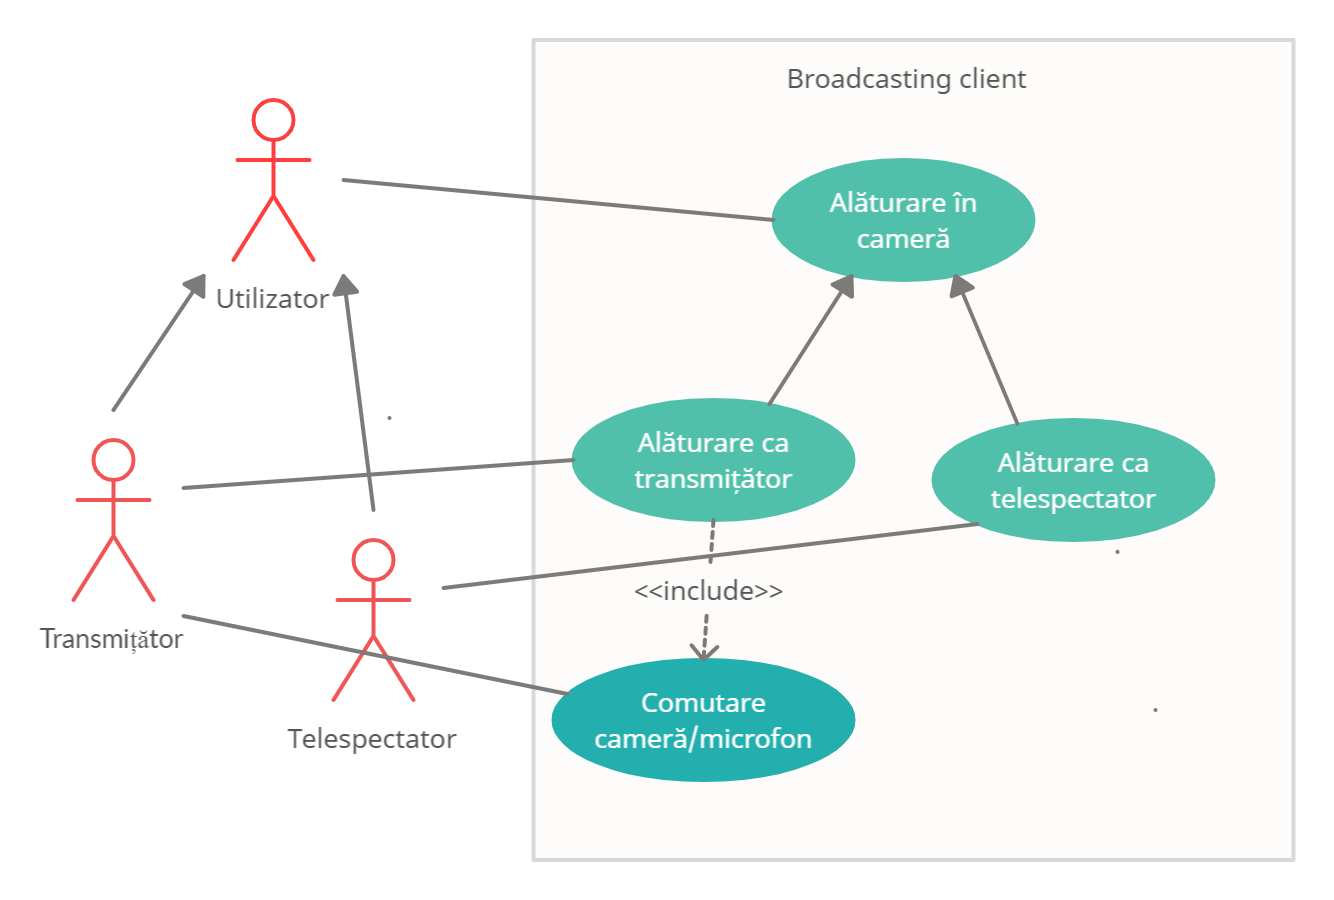
\includegraphics[width=12cm]{figures/app_use_case_diagram.png}
    \caption{Diagrama cazurilor de utilizare}
\end{figure}

\section{Design}
\label{chap:ch6sec2}
\begin{figure}[!htbp]
    \centering
    \scalebox{0.65}{\input{figures/app_linked_topology.pdf_tex}}
    \caption{Topologia înlănțuită folosită de fiecare cameră de pe server}
    \label{AppTopology}
\end{figure}
\indent \par În capitolele anterioare, am discutat despre avantajele și dezavantajele fiecărui tip de topologie în cadrul sesiunilor WebRTC. Am descoperit că o topologie mesh aduce avantajul costurilor de întreținere mai mici, datorită lipsei necesității unui server, dar cu compromisul consumului de resurse ridicat pe fiecare nod. De asemenea, serverele media, datorită centralizării locului de transmisie pentru fiecare nod, aduc avantajul ocupării unei lățimi reduse de bandă, ceea ce permite o compresie redusă a imaginii și a sunetului.
\indent \par Există situații în care latența nu este importantă și unde predomină o singură cameră web pornită, unde participanții nu sunt interactivi. Acestea includ: piesele de teatru, concertele, conferințele de lansare a unui produs. În aceste cazuri, vorbim de un scenariu numit broadcasting. Realizat într-o manieră mesh (unul către toți), ar fi ineficient din punct de vedere al resurselor utilizate și a lățimii de bandă, chiar dacă latența este redusă.
\indent \par Pentru aceasta, în aplicația implementată de mine, fiecare cameră reprezintă o topologie de tip lanț, în care nodurile din capete au un singur vecin, iar restul câte doi. Transmisia se va începe de la un capăt și se va termina la celălalt.
\indent \par Diagrama \ref{AppTopology} nu ne dă informații legate de calitatea conexiunii fiecărui client, așadar conexiunile trebuie evaluate. O modalitate simplă este de a testa viteza de descărcare a unui fișier de dimensiuni suficient de mari încât să se descarce rapid pe conexiunile bune. Pentru conexiunile slabe, nu are rost să așteptăm mai mult de 4 secunde, deoarece alăturarea la o cameră va dura mult în acest caz. Un algoritm simplu în JavaScript ar arăta astfel:
\begin{lstlisting}
export const getAverageDownloadSpeed = async () => new Promise((resolve, reject) => {
    const formData = new FormData()
    formData.append('filetype', 'mp3')
    formData.append('filename', 'test')
    formData.append('filesize', 10485760)
  
    let count = 0
    let sum = 0
    let previousDownloadedAmount = 0
    let previousTime = Date.now()
    const request = new XMLHttpRequest()
    request.onprogress = e => {
      const time = Date.now()
      count++
      sum += (e.loaded - previousDownloadedAmount) / (time - previousTime)
      previousDownloadedAmount = e.loaded
      previousTime = time
    }
    const ultimate = setTimeout(() => {
      request.abort()
      resolve(sum / count)
    }, 4000)
  
    request.open('POST', 'https://cors-anywhere.herokuapp.com/https://www.fakefilegenerator.com/download.php')
    request.send(formData)
    request.onreadystatechange = function () {
      if (request.readyState === 4) {
        if (request.status && request.status !== 200) {
          reject(new Error('Request to https://www.fakefilegenerator.com/download.php returned ' + request.status))
        }
        clearTimeout(ultimate)
        resolve(sum / count)
      }
    }
  })
\end{lstlisting}
\indent \par De observat este funcția \texttt{onprogress} din XMLHttpRequest. Aceasta are rolul de a semnala un progres în returnarea datelor de la cerere. Conține un parametru de tip obiect ce va conține câmpurile \textit{loaded} și \textit{total}. Noi vom avea nevoie de câmpul \textit{loaded} pentru a observa cantitatea descărcată la momentul respectiv. Folosind variabile pentru valorile anterioare atât de cantitate, cât și de timp, vom calcula viteza cu care s-a descărcat porțiunea respectivă. Media acestor viteze va fi returnată de către promise. 
\indent \par Vom folosi un timeout pentru o funcție care va returna forțat media vitezelor în cele 4 secunde scurse, în cazul în care nu se finalizează request-ul HTTPS în timp util. Se va reține în variabila \texttt{ultimate} și va fi eliminat în cazul în care request-ul se termină mai repede.
\indent \par Prima dată, după cum am zis, se va alătura transmițătorul la cameră. El va trimite la server mesajul \texttt{[request]rtc:room:join}. Lui i se va crea în memorie un room nou, o topologie nouă și un nod nou (instanță de RTCClientNode). UUID-ul (universally unique identifier) generat de server la conectare va fi ID-ul transmițătorului, urmând ca să primească răspunsul \texttt{[response]rtc:joining-as-broadcaster}.
\begin{figure}[H]
    \centering
    \scalebox{0.7}{\input{figures/app_two_peer_connection.pdf_tex}}
    \caption{Diagrama de secvență pentru conectarea a doi clienți}
\end{figure}
\indent \par Vom adăuga nodurile în topologie în ordinea descrescătoare a acestor viteze de descărcare. Însă schimbul de descriptori SDP dintre cei doi vecini actuali se va anula. Serverul de signaling va fi responsabil de a trimite event-ul \texttt{[webrtc]remove-peer} părintelui noului nod pentru a putea adăuga ulterior track-urile audio-video la acesta. Va șterge track-urile către vechiul său fiu, pentru a nu adăuga același track de două ori, aruncând excepție din cauză că track-ul este deja asociat unui sender RTP de date. Va trimite \texttt{[webrtc]make-offer} pentru ca părintele să facă schimb de SDP-uri cu noul fiu, urmând ca fiul, după ce primește minim două track-uri (se consideră că unul e audio și celălalt e video), să interogheze serverul pentru noii săi fii, pe care îi va adăuga îl lista sa reținută local. Va aștepta două track-uri de la părinte, deoarece, altfel, lista de track-uri ar fi incompletă, necesitând un alt schimb de descriptori.
\begin{figure}[H]
    \centering
    \scalebox{0.7}{\input{figures/app_three_peer_connection.pdf_tex}}
    \caption{Diagrama de secvență pentru conectarea a trei clienți}
\end{figure}
\indent \par Schimbul imaginii de la cameră presupune trimiterea de noi track-uri către toți clienții. Este bine de știut că RTCPeerConnection va apela funcția \textit{onnegotiationneeded} la fiecare track scos. Dar folosirea acestei funcții va complica implementarea. Așadar, se vor scoate, mai întâi, toate track-urile către fiu și se va trimite \texttt{[webrtc]send-offer} pentru a forța schimbul de descriptori. Fiul său va trimite, de asemenea, aceeași cerere către fiul său, până când toți fiii vor primi noile track-uri de la broadcaster.
\indent \par Din motive de stabilitate, trebuie tratat și cazul când un client va părăsi camera, fie apăsând un buton de părăsire, fie închizând forțat pagina web. Părintele său va fi semnalat că trebuie să îl elimine din lista sa de vecini, urmând ca serverul să îi trimită cereri de tip \texttt{[webrtc]make-offer} către fiecare fiu al său. Apoi, se va parcurge pe server topologia înlănțuită și se va căuta după UUID-ul său, eliminându-l și legând vecinii între ei și la nivel logic.
\indent \par Diagrama de clase va arăta în felul următor:
\begin{figure}[H]
    \centering
    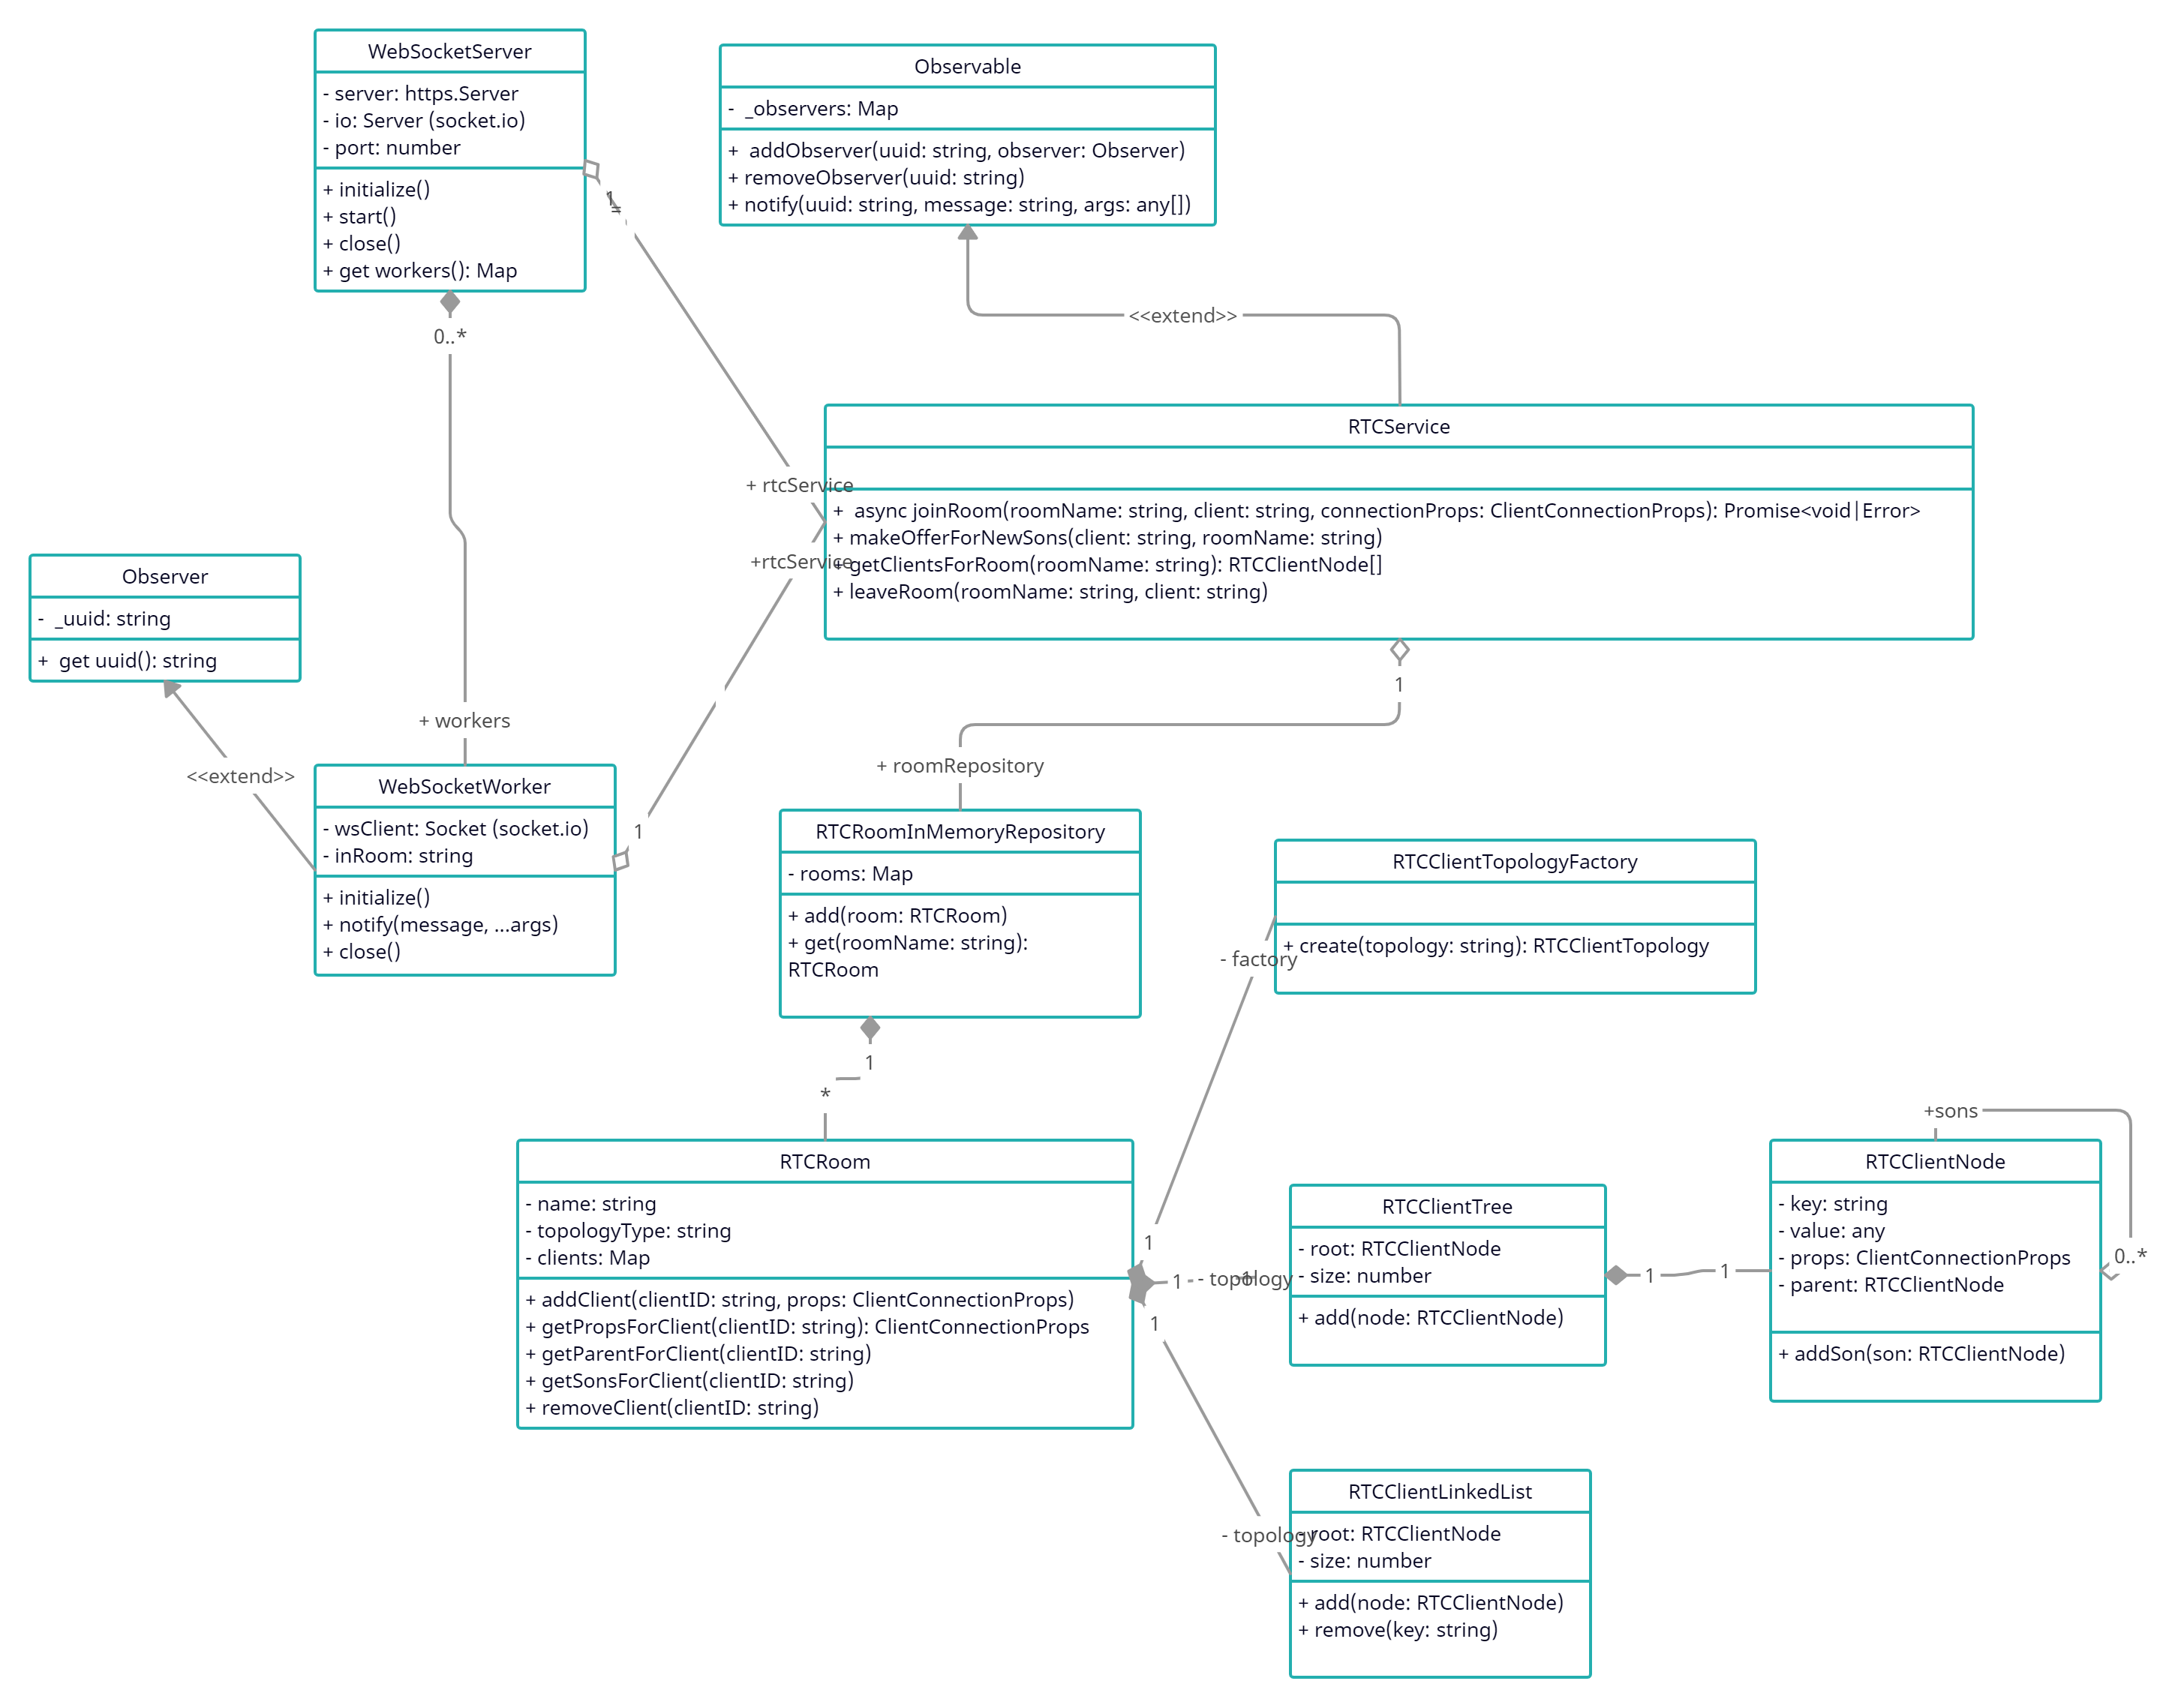
\includegraphics[width=15cm]{figures/app_class_diagram.png}
    \caption{Diagrama de clase a aplicației server}
\end{figure}
\indent \par Se vor folosi și variabile de mediu pentru a reține parametrii necesari:
\begin{itemize}
    \item \textbf{PORT} - portul care va fi deschis pentru ascultarea cererilor;
    \item \textbf{CLIENT\_TOPOLOGY} - topologia care va fi folosită (în acest caz, va fi \textit{list}).
\end{itemize}
\indent \par Pe aplicația clientului, clasa care încapsulează logica menționată mai sus este RTCForwardingPeer. Ea va asculta după toate evenimentele primite de la server și va acționa conform. Include câteva event handlere: pentru schimbarea stării conexiunii WebSocket (inițial va fi \textit{disconnected}, urmând să fie \textit{connected}); pentru primirea unei cereri noi de la nodul părinte (\textit{onParentOffer}), care va fi folosit pentru a opri stream-ul din elementul \textit{video} din componenta VideoBroadcastItem; dar și pentru anunțarea sosirea unui track nou de la părinte, \textit{onTrack}, care va porni redarea stream-ului din elementul \textit{video} menționat anterior.
\indent \par Această clasă va fi îmbrăcată sub formă de hook-uri React în componenta \textit{useWebRTC}. Va fi reactualizată în momentul în care se va schimba room-ul în care va participa, dar și în momentul în care se schimbă starea conexiunii cu serverul.
\begin{figure}[H]
    \centering
    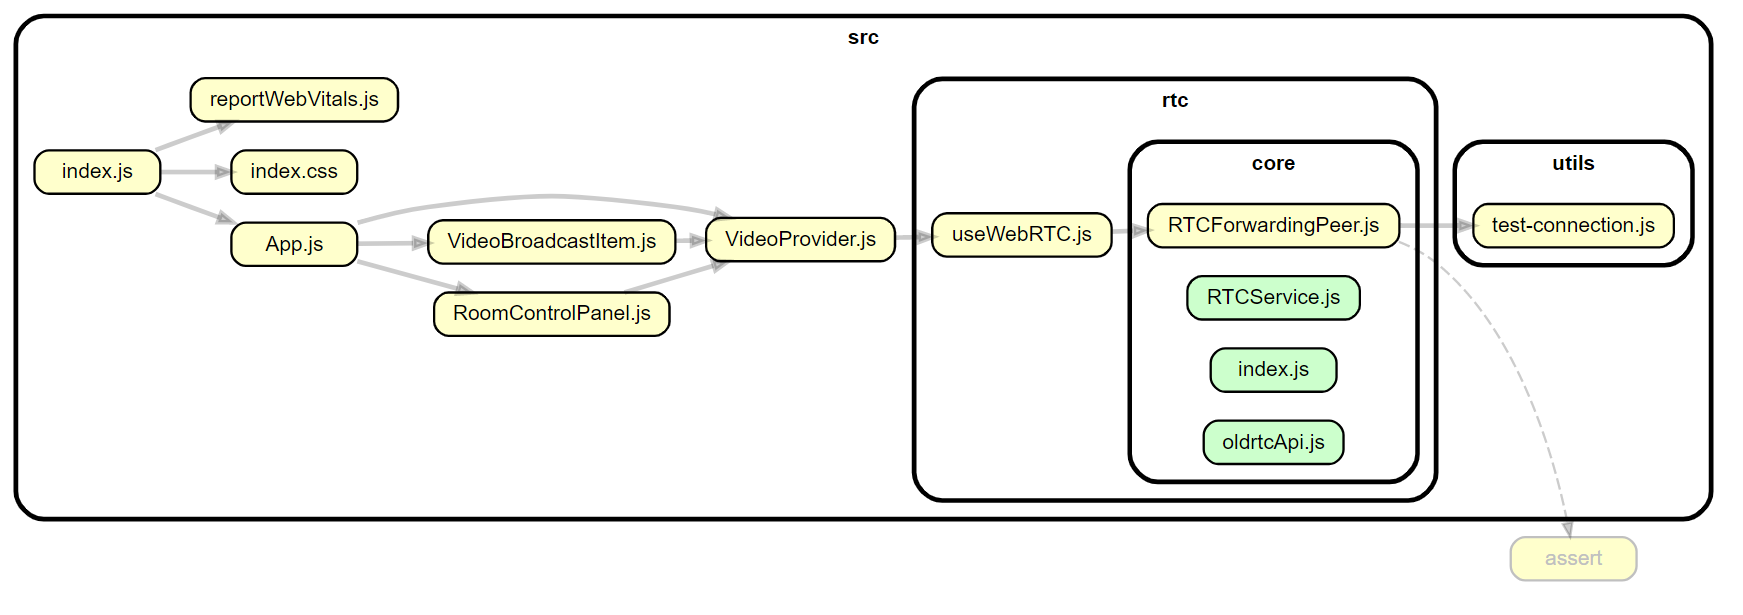
\includegraphics[width=15cm]{figures/app_frontend_dependency_diagram.png}
    \caption{Diagrama de dependințe a aplicației client}
\end{figure}
\section{Utilizare și testare}
\indent \par Utilizatorul, când va deschide aplicația, va fi întâmpinat de această pagină:
\begin{figure}[H]
    \centering
    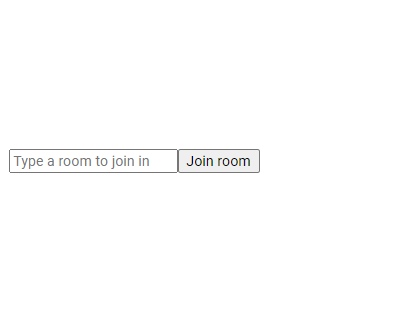
\includegraphics[width=6.5cm]{figures/app_welcome_screen.png}
    \caption{Ecranul principal}
\end{figure}
\indent \par După ce tastează numele unei camere și va apăsa pe butonul \textit{Join room}, va fi întâmpinat cu unul din cele două ecrane:
\begin{figure}[H]
    \centering
    \begin{subfigure}{0.45\textwidth}
        \centering
        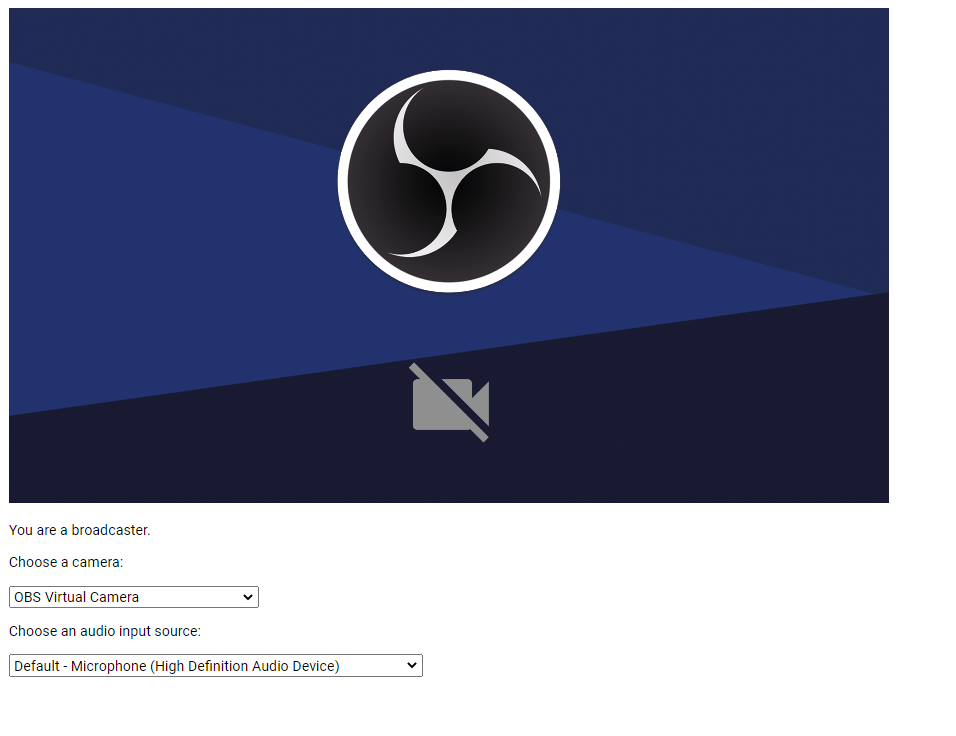
\includegraphics[width=8cm, height=5.5cm]{figures/app_broadcaster_mode.png}
        \caption{Ecranul transmițătorului}
    \end{subfigure}
    \hfill
    \begin{subfigure}{0.45\textwidth}
        \centering
        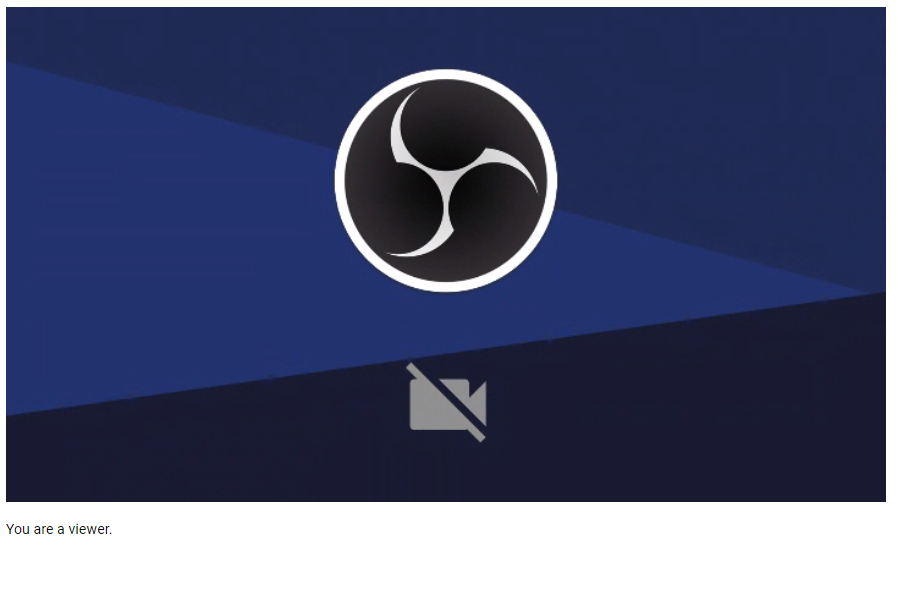
\includegraphics[width=8cm, height=5.5cm]{figures/app_viewer_mode.png}
        \caption{Ecranul spectatorului}
    \end{subfigure}
\end{figure}
\indent \par Transmițătorul poate comuta între camerele web dând click pe meniul cu opțiuni de sub textul \textit{Choose a camera}:
\begin{figure}[H]
    \centering
    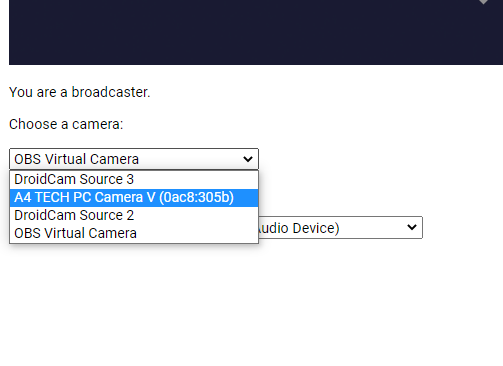
\includegraphics[width=7cm]{figures/app_pick_camera.png}
    \caption{Meniul ce conține lista disponibilă de camere}
\end{figure}
\indent \par Pentru a putea observa lățimea de bandă disponibilă, am afișat în consolă viteza obținută la test. Pe o conexiune pe fir de la Vodafone cu viteză maximă de download de 300 Mbps, am obținut următoarele rezultate:
\begin{figure}[H]
    \centering
    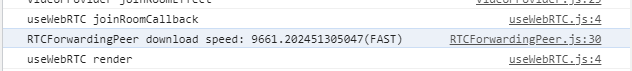
\includegraphics[width=12cm]{figures/app_bandwidth_test.png}
    \caption{Test de lățime de bandă cu rezultatul afișat în consolă (viteza este afișată în KB/s)}
\end{figure}
\begin{figure}[H]
    \centering
    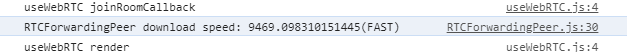
\includegraphics[width=12cm]{figures/app_bandwidth_test_2.png}
    \caption{Al doilea test de lățime de bandă cu rezultatul afișat în consolă}
\end{figure}
\indent \par Am realizat testarea și pe 3 browsere diferite, printre care unul rulând de pe o mașină virtuală cu Linux aflată pe un alt computer. Între transmițător (Microsoft Edge) și Firefox pe Windows, latența observată era minimă, datorită faptului că au rulat pe aceeași mașină, așadar folosind candidații ICE de tip host. Pe Linux, latența era vizibilă.
\indent \par La al doilea test cu același set de browsere, am obținut de la Edge viteza de 127.7740961 KB/s, de la Firefox de pe Linux 606.08179903 KB/s, iar de la cel rulat local pe Windows 258.1044269. Latența imaginii a fost mare pe instanța locală de Firefox, datorită drumului lung care trece prin mașina virtuală. Însă calitatea s-a păstrat identică.
\begin{figure}[H]
    \centering
    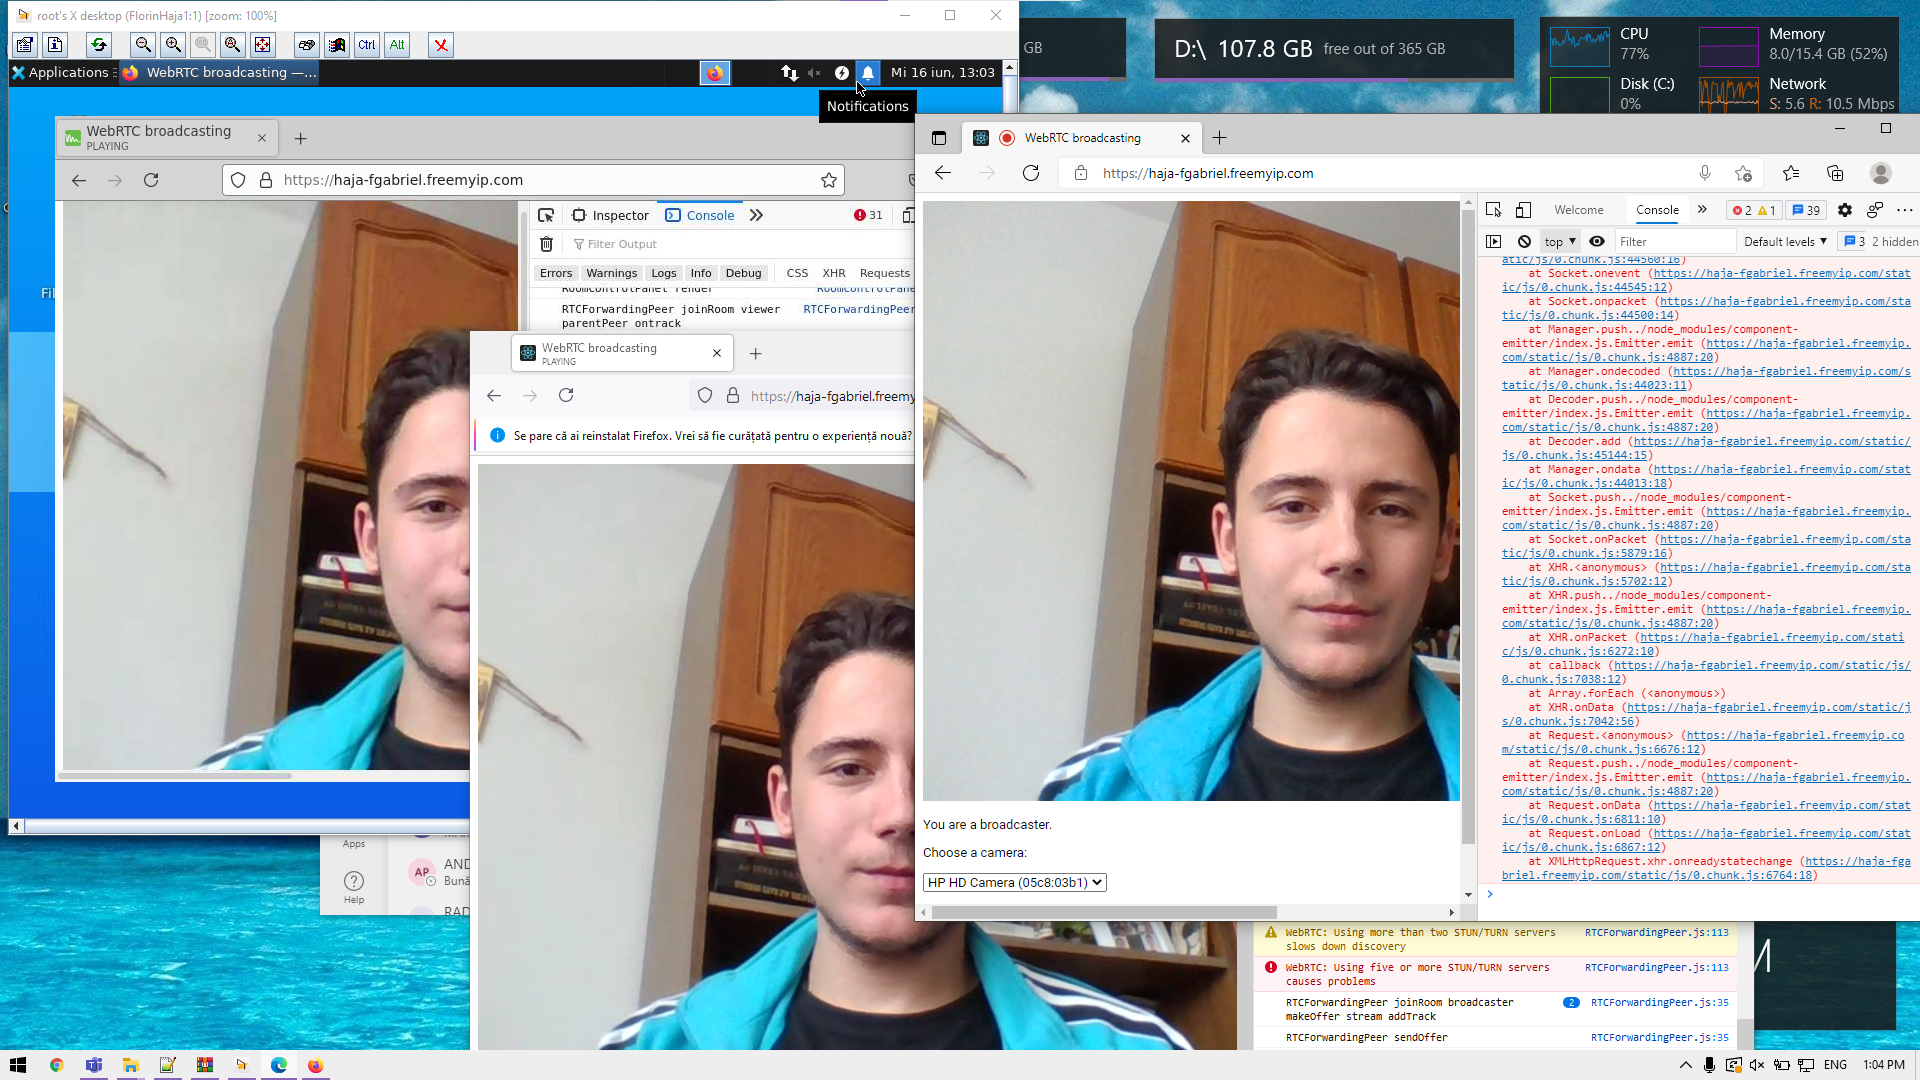
\includegraphics[width=12cm]{figures/app_on_3_browsers.png}
    \caption{Aplicația testată pe 3 browsere diferite: Microsoft Edge pe Windows, Mozilla Firefox pe Windows și Mozilla Firefox pe Linux}
\end{figure}
\indent \par Se poate ține cont și de geolocație, precum și de faptul dacă un spectator se află pe aceeași rețea cu transmițătorul, însă acestea vor fi considerate îmbunătățiri pentru viitor.
\chapter{Concluzii și posibile îmbunătățiri}
%\chapter*{Concluzii}
\label{sec:ch6}

\par Concluzii ...

%\addcontentsline{toc}{chapter}{Concluzii}
%\addcontentsline{toc}{chapter}{Conclusions}

\bibliography{references}

\end{document}
